\section{Architectural Patterns}
This section describes the architectural patterns we will be using when developing this game. Patterns
are useful because they solve problems that occur regularly in projects and it makes it easier for 
others to learn your code, because it solves well known problems using well known methods.

\subsection*{Model-View-Presenter}
This project will primarily be using the Model-View-Presenter pattern for its architecture and will 
be using the JavaScript library Backbone to implement the pattern. Model-View-Presenter is a slightly
modified version of Model-View-Controller, made to work better with HTML and JavaScript. A model is 
an object that stores data. The model also contains the logic for modifying the data it contains. 
A view contains the logic for displaying an object and the Controller contains the logic for 
processing user input and updating the model. The model notifies the view whenever there is a change
to the state of the model. In practice the same object is often both View and Controller. 
Model-View-Presenter embraces this concept. The Presenter is a JavaScript object which connects a 
Backbone Model to the HTML object which serves as the View. 
\cite{mvp}

\begin{figure}[H]
	\centering
	\subfigure{
		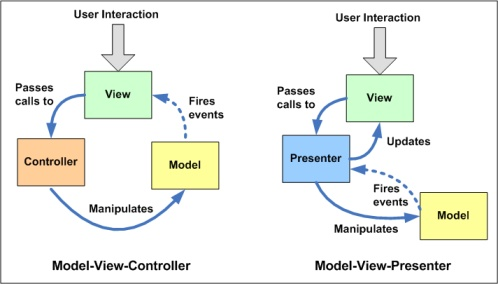
\includegraphics{pictures/mvc_mvp}
	}
	\caption{Comparison between Model-View-Controller and Model-View-Presenter}
\end{figure}

\subsection*{Game Loop}
The game runs a loop using the JavaScript requestAnimationFrame function. This loop updates the parts 
of the game which needs to be updated and repaints the parts of the screen which needs to be repainted.

\subsection*{Singletons}
There are 2 singleton objects in the game. One is an Image Library which is responsible for loading 
and storing the sprites the game will draw to the screen. This will allow us to only read and store 
each sprite one time, saving memory and improving performance. The second singleton object is the 
Object Pool. This object creates game objects, and stores them while they are not placed on the game 
map. This object will create all the objects when the game loads, so that they do not have to be 
created later, further improving performance. The Object Pool also prevents garbage collection from 
reducing the game's performance. Both these singletons are commonly used in video games.
